\documentclass[ucs, notheorems, handout]{beamer}

\usetheme[numbers,totalnumbers,minimal,nologo]{Statmod}
\usefonttheme[onlymath]{serif}
\setbeamertemplate{navigation symbols}{}
\setbeamercolor{alerted text}{fg=blue}

\mode<handout> {
    \usepackage{pgfpages}
    %\setbeameroption{show notes}
    %\pgfpagesuselayout{2 on 1}[a4paper, border shrink=5mm]
    \setbeamercolor{note page}{bg=white}
    \setbeamercolor{note title}{bg=gray!10}
    \setbeamercolor{note date}{fg=gray!10}
}

\usepackage[utf8x]{inputenc}
\usepackage[T2A]{fontenc}
\usepackage[english]{babel}
\usepackage{tikz}
\usepackage{ragged2e}
\usepackage{graphicx}
\usepackage{subfigure}

\usepackage{amsmath}
\usepackage{amsfonts}
\usepackage{amsthm}

\DeclareMathOperator{\med}{med}
\DeclareMathOperator{\diag}{diag}
\DeclareMathOperator{\tr}{tr}
\DeclareMathOperator*{\argmin}{argmin}
\newcommand{\tX}[1]{\mathsf{#1}}

\title[Robust CSSA]
{Robust Versions of the Complex SSA Method}

\subtitle
{}

\author[Senov M.] 
{Senov Mikhail}

\institute{
\small
    St Petersburg University\\
    Department of Statistical Modelling\\
    \vspace{1cm}
Science and Progress}

\date[Conference]{St Petersburg, November 9, 2021}


\begin{document}

\begin{frame}
  \titlepage
  \note{}
\end{frame}

\begin{frame}{Introduction: Problem}

$\tX{X}_N = (x_1, \ldots, x_{N})$ time series, $N$ series length.\\
\vspace{1em}
\alert{Model:} $\tX{X}_N = \tX{S}_N + \tX{R}_N$, $\tX{S}_N$ signal, $\tX{R}_N$ noise.\\
\vspace{1em}
\alert{Problem:} Signal extraction $\tilde{\tX{S}} = F(\tX{X}_N)$, $F$ is used method.\\
\vspace{1em}
\alert{Method:} SSA (Singular Spectrum Analysis) [Analysis of Time Series
Structure: SSA and Related Techniques, Golyandina N., Nekrutkin V.,
Zhigljavsky A., 2001].

    \note{}
\end{frame}

\begin{frame}{Introduction: Time series with outliers and SSA}
Basic SSA: reacts to outliers.
\begin{center}
    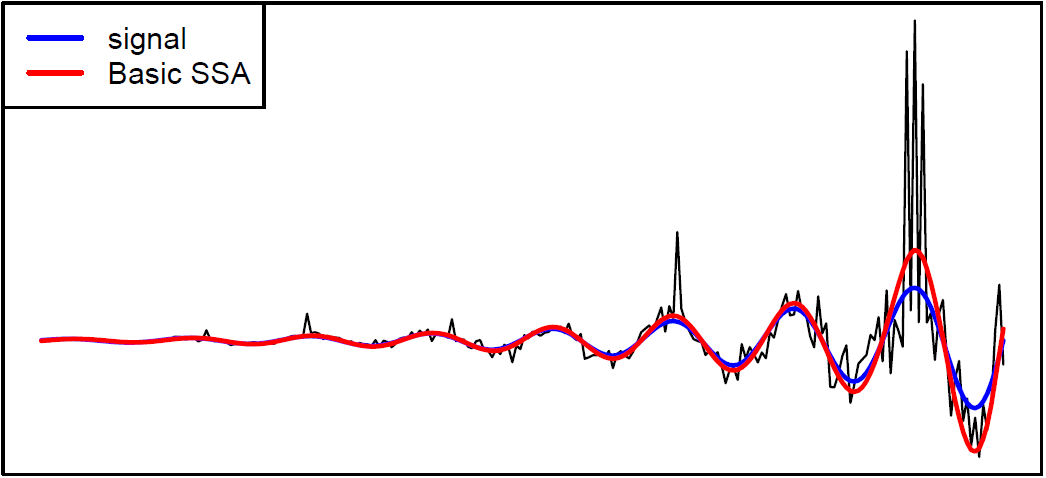
\includegraphics[, height = 3cm]{otliers_ssa.PNG}
\end{center}

Robust SSA: does not reacts to outliers.
\begin{center}
    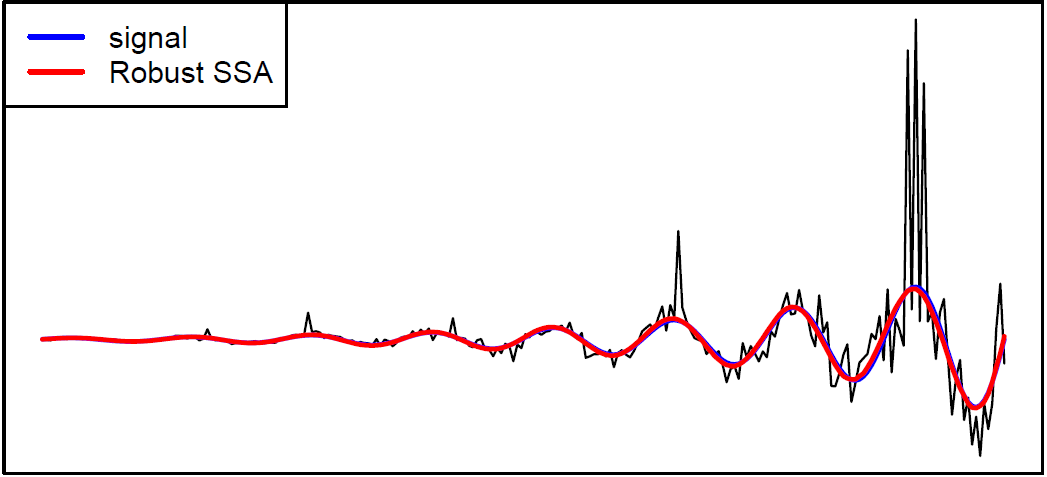
\includegraphics[, height = 3cm]{outliers_l1.PNG}
\end{center}

    \note{}
\end{frame}

\begin{frame}{Introduction: Aim of the talk}
    Robust SSA is developed for real-valued time series.\\
    \vspace{1em}
    \alert{Aim:} Generalize Robust SSA to the complex-valued time series case.\\
    \vspace{1em}
   Common example of complex time series is engineering tasks where data are produced by Fourier transform.
   $$\tX{X}_N^{(t)} = (x_1^{(t)}, \ldots, x_N^{(t)}), \, t = 1 \ldots M,$$
   $$\tX{DFT}(\tX{X}_N^{(t)}) = f^{(t)}_k = \sum_{n=1}^{N}x^{(t)}_n e^{-2 \pi i k  n / N}, \, k = 1 \ldots N,$$
   $$\tX{F}^{(M)}_{k} = (f^{(1)}_k, \ldots, f^{(M)}_k).$$
\end{frame}


\begin{frame}{Methods: Notations}
Consider the time series $\tX{X}_N=(x_1, \ldots, x_{N})$.\\
\vspace{1em}
$\mathcal{M}_{\mathcal{H}}$~--- space of hankel matrix $L\times K$,

$\mathcal{M}_{r}$ --- space of matrix of rank at most $r$,  $L \times K$.\\
\vspace{1em}
Embedding operator $\mathcal{T}:\mathbb{R}^N \rightarrow \mathcal{M}_{\mathcal{H}}: \mathcal{T} (\tX{X_N}) = \mathbf{X} $,\\
\vspace{1em}
$\Pi_{r}:\mathcal{M}\rightarrow \mathcal{M}_r$~--- projector onto the space of matrices of rank at most $r$ in some norm in the matrix space,\\
\vspace{1em}
$\Pi_{\mathcal{H}}:\mathcal{M} \rightarrow \mathcal{M}_{\mathcal{H}}$~--- projector onto the space of hankel matrices in some norm in the matrix space.

    \note{}

\end{frame}

\begin{frame}{Methods: Signal extraction}

Time series $\tX{X}_N=(x_1, \ldots, x_{N})$.
\begin{block}{Algorithm for signal extraction}
\begin{equation*}
	\tilde{\tX{S}} = \mathcal{T}^{-1} \Pi_{\mathcal{H}} \Pi_{r} \mathcal{T} (\tX{X_N}).
\end{equation*}
\end{block}


Norms for both $\Pi_r$ and $\Pi_{\mathcal{H}}$:
\begin{itemize}
        \item $\mathbb{L}_2$(Frobenius). Basic SSA signal extraction.
        \item $\mathbb{L}_1$. Robust SSA version.
        \item weighted $\mathbb{L}_2$. Robust SSA version.
\end{itemize}
    \note{}
\end{frame}


\begin{frame}{Methods: Illustrative example}
    \begin{block}{Example}
    $(x_1, \ldots, x_N)$, norm $p(x)$, $\argmin\limits_{c}p((x_1 - c, \ldots, x_N - c)) =\, ?$
    \end{block}
    Norms:
    \begin{itemize}
        \item $\mathbb{L}_2$. $\overline{x} = \argmin\limits_{c} \sqrt{\sum_{i = 1}^{N} |x_i - c|^2}$. \\
        If $x_i \to \infty$, then $\overline{x} \to \infty$. Non-robust.
        \item $\mathbb{L}_1$. $\med = \argmin\limits_{c} \sum_{i = 1}^{N} |x_i - c|$. \\
        If $x_i \to \infty$, then $\med \not\to \infty$. Robust.
        \item weighted $\mathbb{L}_2$. $\overline{x}_w = \argmin\limits_{c} \sqrt{\sum_{i = 1}^{N} w_i|x_i - c|^2}$.\\
        If $x_i \rightarrow \infty$, then $w_i = 0$ and $\overline{x}_w \not\to \infty$. Robust.
    \end{itemize}
\end{frame}

\begin{frame}{$\mathbb{L}_2$ CSSA (Basic)}
    Trajectory matrix $\mathbf{Y} \in \mathbb{C}^{L\times K}$ as input.\\
    \vspace{1em}
    $\mathbf{X}^{\mathrm{H}} = \overline{\mathbf{X}^{\mathrm{T}}}$.
    \begin{block}{Problem}
    \begin{equation*}
	    \|\mathbf{Y}-\mathbf{M}\mathbf{V}^{\mathrm{H}}\|_F^2 \longrightarrow \min_{\mathbf{M},\mathbf{V}}, \, \mathbf{M} \in \mathbb{C}^{L\times r}, \mathbf{V} \in \mathbb{C}^{K\times r}
    \end{equation*}
    \end{block}
    $$\tX{SVD}(\mathbf{Y}) = \sum_{i = 1}^{r} \sqrt{\lambda_i}U_i V_i^{\mathrm{H}} = \mathbf{U} \mathbf{\Lambda} \mathbf{V}^{\mathrm{H}},$$
    $U_i$ eigenvector of $\mathbf{Y} \mathbf{Y}^{\mathrm{H}}$, $\lambda_i$ $i$-th eigenvalue of $\mathbf{Y} \mathbf{Y}^{\mathrm{H}}$, $V_i$~eigenvector of $\mathbf{Y}^{\mathrm{H}} \mathbf{Y}$.\\
    \vspace{1em}
    There is closed-from solution $\mathbf{M}\mathbf{V}^{\mathrm{H}}$, $\mathbf{M} = \mathbf{U} \mathbf{\Lambda}$.

    \note{}
\end{frame}

\begin{frame}{$\mathbb{L}_1$ CSSA}

Trajectory matrix $\mathbf{Y} \in \mathbb{C}^{L\times K}$ as input.
\begin{block}{Problem}
\begin{equation*}
	\|\mathbf{Y}-\mathbf{M}\mathbf{V}^{\mathrm{H}}\|_1 \longrightarrow \min_{\mathbf{M},\mathbf{V}}, \, \mathbf{M} \in \mathbb{C}^{L\times r}, \mathbf{V} \in \mathbb{C}^{K\times r}
\end{equation*}
\end{block}
There is no closed-from solution. Solve it iteratively 
\begin{equation*}
	 \mathbf{M(t)} = \argmin\limits_{\mathbf{M}\in \mathbb{C}^{L\times r}} \|\mathbf{Y} - \mathbf{M}\mathbf{V}^\mathrm{H}(t - 1)\|_1
\end{equation*}
$$\mathbf{V(t)} = \argmin\limits_{\mathbf{V}\in \mathbb{C}^{K\times r}} \|\mathbf{Y} - \mathbf{M}(t)\mathbf{V}^\mathrm{H}\|_1.$$

Can be reduced to the linear case and solved by evaluating weighted-median.

    \note{}
\end{frame}


\begin{frame}{Weighted $\mathbb{L}_2$ CSSA: Algorithm}

Trajectory matrix $\mathbf{Y} \in \mathbb{C}^{L\times K}$ as input.\\ 
\vspace{1em}
Iteratively compute matrix of weights $\mathbf{W} \in \mathbb{R}^{L\times K}$ .
\begin{block}{Problem}
\begin{equation*}
	\|\mathbf{W}^{1/2}\odot(\mathbf{Y}-\mathbf{M}\mathbf{V}^{\mathrm{H}})\|^{2}_F \longrightarrow \min_{\mathbf{M},\mathbf{V}}, \, \mathbf{U} \in \mathbb{C}^{L\times r}, \mathbf{V} \in \mathbb{C}^{K\times r}
\end{equation*}
\end{block}
There is not closed-from solution. Solve it iteratively
\begin{equation*}
	\mathbf{M(t)} = \argmin\limits_{\mathbf{M}\in \mathbb{C}^{L\times r}} \|\mathbf{W}^{1/2}\odot(\mathbf{Y}-\mathbf{M}\mathbf{V}^{\mathrm{H}}(t-1))\|^2_F
\end{equation*}
$$\mathbf{V(t)} = \argmin\limits_{\mathbf{V}\in \mathbb{C}^{K\times r}} \|\mathbf{W}^{1/2}\odot(\mathbf{Y}-\mathbf{M}(t)\mathbf{V}^{\mathrm{H}})\|^2_F$$
Can be reduced to the IRLS.

    \note{}
\end{frame}

\begin{frame}{Weighted $\mathbb{L}_2$ CSSA: Weights computation}
Outliers are determined by their absolute value.
    \begin{block}{Algorithm}
    \begin{enumerate}
        \item Residuals matrix computing $\mathbf{R} = \{r_{ij}\}_{i,j=1}^{n,p} = \mathbf{Y} - \mathbf{M}\mathbf{V}^\mathrm{H}$
        \item Updating matrix $\mathbf{\Sigma} =      \{\sigma_{ij}\}^{L,K}_{i,j=1}$
        \item Computing weights $\mathbf{W} = \{w_{ij}\}^{L,K}_{i,j=1} = \{w(\frac{r_{ij}}{\sigma_{ij}})\}^{L,K}_{i,j=1}$, using
        $$w(x) = 
        \begin{cases}
        (1 - (\frac{|x|}{\alpha})^2)^2 &|x| \leq \alpha\\
        0 &|x| > \alpha\\
        \end{cases}$$
    \end{enumerate}    
    \end{block}
    Algorithm similar to loess method.
    \note{}
\end{frame}

\begin{frame}{Weighted $\mathbb{L}_2$ CSSA: Heteroscedastic noise specifics}
     Consider time series with heteroscedastic noise.
     \begin{center}
        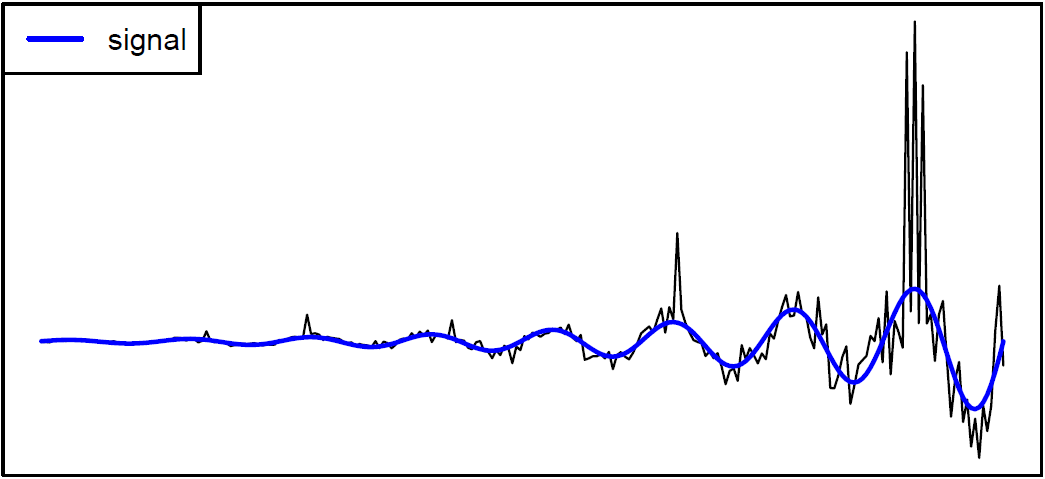
\includegraphics[, height = 3cm]{signal.PNG}
    \end{center}
     Right-sided non-outliers is bigger than left-sided outliers.\\
     \vspace{1em}
     \alert{Basic:} Normalizing coefficient $\sigma_{ij}$ is the same for each series element. Outliers determination is incorrect.\\
     \vspace{1em}
     \alert{Modification:} Compute $\sigma_{ij}$ as trend of residual series.
\end{frame}

\begin{frame}{Implementations}
    \alert{Basic CSSA}: R-package Rssa (Korobeynikov et al, 2020)\\
    \vspace{1em}
    \alert{L1 CSSA}: Was implemented in R language.\\
    \vspace{1em}
    \alert{Weighted L2 CSSA}: Was implemented in R language using real-valued implementation (Tretyakova, 2020).\\
    \vspace{1em}
    A typo that was essential for the weighted $\mathbb{L}_2$ implementation was found in article (Chen et al, 2015) and corrected.
    \begin{figure}[ht]
    \subfigure[Re]{
    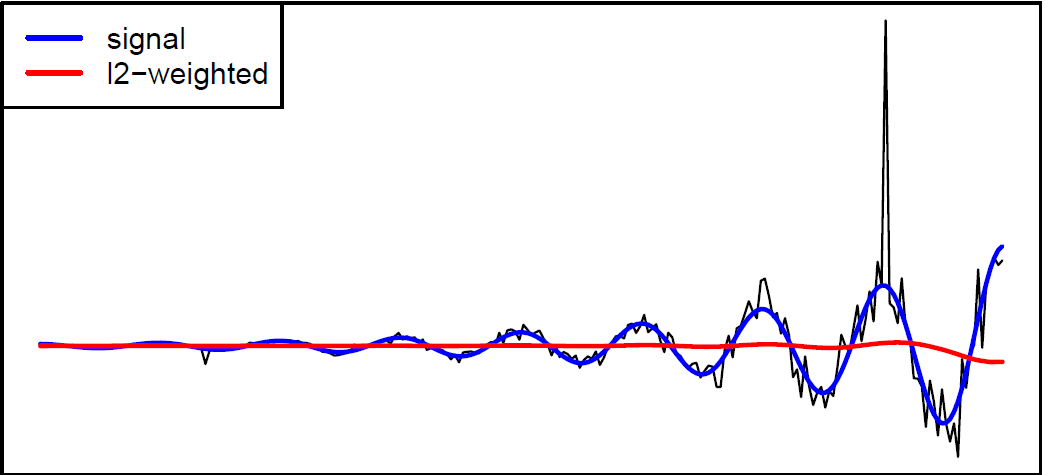
\includegraphics[, height = 2cm]{bad_re.PNG}
    }
    \subfigure[Im]{
    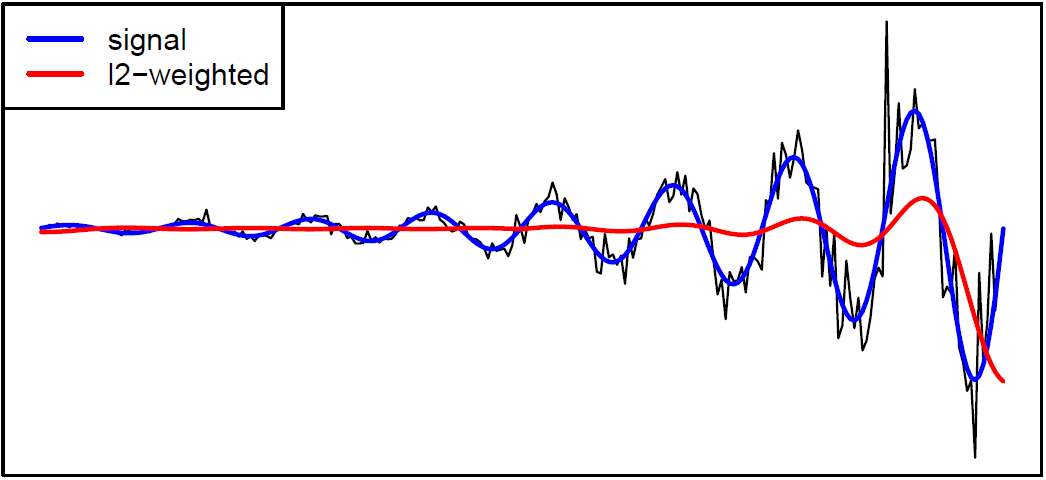
\includegraphics[, height = 2cm]{bad_im.PNG}
    }
    \caption{weighted $\mathbb{L}_2$ version with typo}
    \end{figure}
\end{frame}

\begin{frame}{Example: Time series}
    Motivation:
    \begin{itemize}
        \item Demonstrate that Robust versions better than basic CSSA for some series with outliers.
        \item Demonstrate that modified weighted $\mathbb{L}_2$ version is better than the unmodified one for the case of heteroscedastic noise.
    \end{itemize}
    \vspace{1em}
    \alert{Example}:
    Time series of length $N = 240$ with heteroscedastic noise,
    $$f_n = e^{4n/N} e^{2n\pi/30i} + \frac{1}{2}e^{4n/N} \varepsilon_n, ~ \varepsilon_n \sim CN(0,1),$$
    with $0\%$ outliers and $5\%$ outliers with outlier value $5f_i$.
\end{frame}

\begin{frame}{Example: RMSE comparison}
    \begin{table}[H]
	\begin{center}
		\caption{RMSE of different methods}
		\label{tab3}
		\begin{tabular}{|c|c|c|c|c|}
			\hline
			Outliers & L2 & L1 & w-L2 & mod. w-L2 \\ 
			\hline
			0\% & \textbf{1.28}  & 1.52  & 1.90 & 1.36 \\
			\hline
			5\% & 6.14  & 1.78  & 1.66 & \textbf{1.48} \\
			\hline
		\end{tabular}
	\end{center}
    \end{table}

All comparisons with the \textbf{best} meaningful for $\alpha = 0.05$.\\
\vspace{1em}
Example conclusions:
\begin{itemize}
    \item Basic CSSA demonstrates the best result without outliers,
    \item Robust versions demonstrates significantly better result than basic CSSA with outliers,
    \item Modified method shows better result than unmodified for heteroscedastic noise.
\end{itemize}
\end{frame}

\begin{frame}{Conclusions}
    \begin{itemize}
        \item Robust SSA versions were generalized to the complex-valued case.
        \item Complex Robust SSA versions were implemented in R language.
        \item Example demonstrating the effectiveness of the methods was considered. 
    \end{itemize}
\end{frame}

\end{document}
